\documentclass[a4paper]{book}
%\pagestyle{page}
\usepackage{graphicx}
\usepackage{html}
\usepackage{ifpdf}
\usepackage{fancyhdr}
\usepackage[utf8]{inputenc}
\usepackage{amssymb,amsmath}
\newcommand{\mbf}[1]{\mbox{\boldmath$#1$}}
\font\mbff=cmbsy10\def\mbfx#1{\hbox{\mbff#1}}%\let\mbf\Mbff
\newcommand{\del}[2]{\mbox{$\displaystyle\frac{#1}{#2}$}}
\newcommand{\pard}[2]{\del{\partial \,{#1}}{\partial \,{#2}}}
\newcommand{\ppd}[2]{\del{\partial \,{#1}}{\partial \,{#2}}}
\newcommand{\dpd}[2]{\del{\partial ^{2}\,{#1}}{\partial \,{#2}^{2}}}
\newcommand{\tpd}[2]{\del{\partial ^{3}\,{#1}}{\partial \,{#2}^{3}}}
\newcommand{\cpd}[2]{\del{\partial ^{4}\,{#1}}{\partial \,{#2}^{4}}}
%\newcommand{\spd}[1]{\del{\partial ^{3}\,{#1}}{\partial \,x\,\partial \,t^{2}}}
%\newcommand{\scpd}[1]{\del{\partial ^{4}\,{#1}}{\partial \,x^{2}\,\partial
%\,t^{2}}}
\newcommand{\der}[2]{\del{d \,{#1}}{d \,{#2}}}
\newcommand{\dd}[2]{\del{d ^2\,{#1}}{d \,{#2}^2}}
\newcommand{\td}[2]{\del{d ^3\,{#1}}{d \,{#2}^3}}
\newcommand{\cd}[2]{\del{d ^4\,{#1}}{d \,{#2}^4}}
\newcommand{\MKP}{{MKP$\;\;$}}
\newcommand{\inl}[2]{\mbox{$\displaystyle\int_{#1}^{#2}$}}
\newcommand{\sul}[2]{\mbox{$\displaystyle\sum_{#1}^{#2}\,$}}
\newcommand{\limit}[1]{\mbox{$\displaystyle\lim_{#1}$}}
\newcommand{\vp}{\varphi}
\newcommand{\e}{\mbf{\varepsilon}}
\newcommand{\ep}[0]{\mbf{\varepsilon}^p}
\newcommand{\epd}[0]{\dot{\mbf{\varepsilon}}^p}
\newcommand{\sig}{\mbf{\sigma}}
\newcommand{\sigs}{\sigma}%scalar
\newcommand{\kap}{\mbf{\kappa}}

\newcommand{\vsigrate}{\dot {\mbf{\sigma}}}
\newcommand{\sigrate}{\dot {\sigma}}
\newcommand{\taurate}{\dot {\tau}}
\newcommand{\erate}  {\dot {\mbf{e}}}

\newcommand{\rest}[1]{\Re\left( {#1} \right)}
\newcommand{\refeq}[1]{Eq.~(\ref{#1})}
\newcommand{\reffig}[1]{Fig.~(\ref{#1})}
\newcommand{\refeqs}[2]{Eqs.~(\ref{#1}), (\ref{#2})}
\newcommand{\refeqsr}[2]{\mbox{Eqs.~(\ref{#1})-(\ref{#2})}}

\newcommand{\C}{$^{\circ}\mathrm{C}$}
\newcommand{\ymu}{y_{\mu}}
\newcommand{\y}[1]{y_{#1}}
\newcommand{\ymui}[1]{y_{\mu_{#1}}}
\newcommand{\tdymu}{{\dot y}_{\mu}}
\newcommand{\ttdymu}{{\ddot y}_{\mu}}
\newcommand{\timeder}[1]{\dot {#1}} 
\newcommand{\dprime}{\prime\prime}

\newcommand{\beq}{\begin{equation}}
\newcommand{\eeq}{\end{equation}}
\newcommand{\bea}{\begin{eqnarray}}
\newcommand{\eea}{\end{eqnarray}}
\newcommand{\vsi}{\mbf{\sigma}}
\newcommand{\vep}{\mbf{\varepsilon}}
\newcommand{\eps}{\varepsilon}
\newcommand{\mD}{\mbf{D}}
\newcommand{\vxi}{\mbf{\xi}}
\newcommand{\vx}{\mbf{x}}
\newcommand{\dxi}{\;\mbox{d}\mbf{\xi}}
\newcommand{\vf}{\mbf{f}}
\newcommand{\vg}{\mbf{g}}
\newcommand{\veps}{\mbf{\varepsilon}}
\newcommand{\mB}{\mbf{B}}
\newcommand{\vsig}{\mbf{\sigma}}
\newcommand{\vd}{\mbf{d}}
\newcommand{\mK}{\mbf{K}}
\newcommand{\macbra}[1]{\langle{#1}\rangle}
\newcommand{\vbs}{\mbf{b}^{\sigma}}
\newcommand{\vbe}{\mbf{b}^{\eta}}
\newcommand{\vbeT}{\mbf{b}^{\eta T}}

\newcommand{\ud}{\mathrm{d}}
\newcommand{\grad}{\nabla}
%position vectors
\newcommand{\x}{\mbf{x}}
\newcommand{\xd}{\mbf{x}^\varphi}
%displacement
\newcommand{\du}{\mbf{u}} 
\newcommand{\bestresultcolor}{blue}
\newcommand{\bestresult}[1]{\textcolor{\bestresultcolor}{\bf{#1}}}
\newcommand{\ignore}[1]{}





\newcommand{\oofem}{\htmladdnormallink{OOFEM}{http://www.oofem.org}\ }
\newcommand{\oofemlnk}[1]{\htmladdnormallink{#1}{http://www.oofem.org}\ }
\newcommand{\bp}{\htmladdnormallink{Bo\v{r}ek Patz\'{a}k}{http://mech.fsv.cvut.cz/~bp/bp.html}}



\oddsidemargin -10mm
\evensidemargin -10mm
\textwidth 180mm
\parindent 0mm

\begin{document}
%begin{latexonly}
\title{
\ifpdf
\oofemlnk{\centerline{
\includegraphics[width=0.7\textwidth]{figs/oofem-logo-contour.pdf}}}
\else
\oofemlnk{\centerline{
\includegraphics[width=0.7\textwidth]{figs/oofem-logo-contour.eps}}}
\fi
Theory manual}
\author{Bořek Patzák, Martin Horák, Filip Kolařík\\ \\
Czech Technical University\\
Faculty of Civil Engineering\\
Department of Structural Mechanics\\
Th\'akurova 7, 166 29 Prague, Czech Republic
}
\maketitle
%end{latexonly}
\begin{htmlonly}
\begin{center}
\oofemlnk{\centerline{
\includegraphics[width=0.7\textwidth]{figs/oofem-logo-contour.eps}}}
{\Large Theorz manual}\\ \\
{Bořek Patzák, Martin Horák, Filip Kolařík\\ 
Czech Technical University\\
Faculty of Civil Engineering\\
Department of Structural Mechanics\\
Th\'akurova 7, 166 29 Prague, Czech Republic
}
\end{htmlonly}

\section*{Acknowledgments}
This work was supported by the Grant Agency of the Czech Republic -
Project No.: 103/97/P106.

\clearpage
%\setcounter{page}{1}
\pagestyle{headings}

\tableofcontents
\chapter{Introduction and basic equations}
\section{Introduction}
% Section: Introduction
The aim of this document is to ducument the theoretical bacground of available solvers, elements, and models in oofem. At present, this manual is a working document, covering only small portion of its capabilities.  

\subsection{Notation}
\begin{table}[h!]
  \begin{center}
  \begin{tabular}{|l|p{8cm}|}
    \hline
    $\mbf{B}^e$ & Element strain-displacement matrix\\
    $\mbf{C}$ & Elastic constitutive matrix\\
    $\mbf{r}$ & Displacement vector\\
    $\mbf{r}^e$ & Element displacement vector\\
    $\hat{\mbf{r}}$ & Global displacement vector\\
    $\mbf{K}$ & Stiffness matrix\\
    $N_i^e$ & Element shape function\\
    $\mbf{n}$ & Exterior unit normal vector\\
    $\Gamma$ & Domain boundary\\
    $\Gamma_u$ & Dirichlet boundary\\
    $\Gamma_t$ & Neumann boundary\\
    $\delta_{ij}$ & Kronecker symbol\\
    $\mbf{\eps}$ & Infinitesimal deformation tensor\\
    $\nu$ & POisson's ratio\\
    $\mbf{\sigma}$ &Cauchy stress tensor\\
    \hline
  \end{tabular}
  \end{center}
  \caption{Table of symbols}
\end{table}

% Basic equations
\section{Linear elasticity}
\subsection{Linear kinematics}
Let us consider a deformable body as a collection of points, where position of each point is denoted as $\x\in\Omega$. In a deformed configuration the position of each point is identified by its position vector $\xd(x) = \mbf{\phi}(\x)$. The displacement vector is then defined as:
\begin{equation}
  \label{eq:displacementvector}
  \xd(\x) = \x + \du(\x)  
\end{equation}

Let us now examine the position in a local neighborhood of a point. The deformed position of such neighbor point with coordinates $\x+d\x$ (where d\x is infinitisemally small vector) is
$$\xd(\x+d\x) = \x+d\x+\du(\x+d\x) = \xd + d\xd$$,
where $d\xd$ is the mapping of vector $d\x$ onto deformed configuration, see Fig.~\ref{fig:deformedconfiguration}.
\begin{figure}
  \begin{center}
    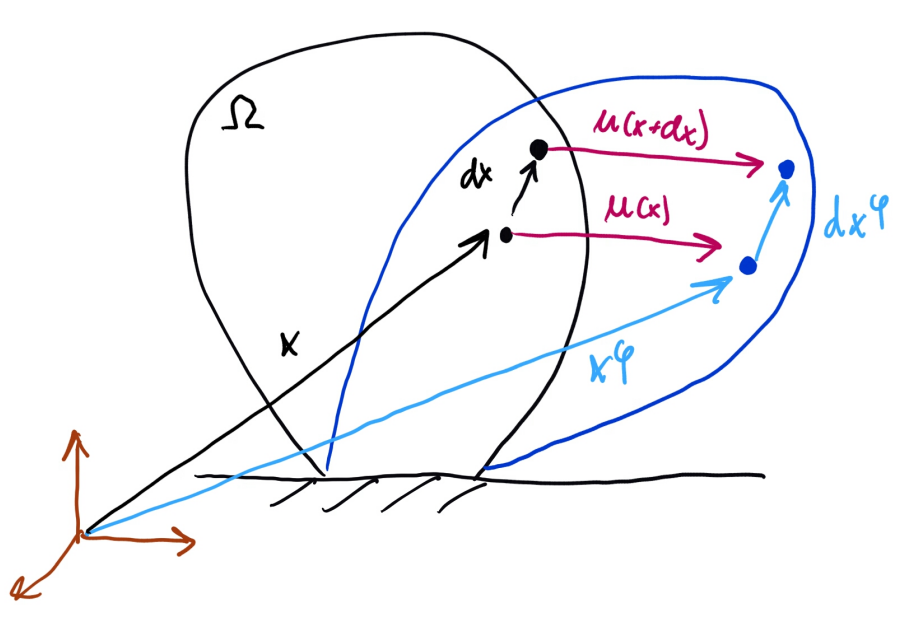
\includegraphics[width=0.5\textwidth]{figs/deformedconfiguration.png}
  \end{center}
  \label{fig:deformedconfiguration}
  \caption{Deformed configuration}
\end{figure}
Taking into account the definition of displacement vector ~\ref{eq:displacementvector} and using Taylor formula we get
\begin{equation}
  d\xd = \x+d\x+\du(\x+d\x)-\xd = d\x-\du(\x)+\du(\x+d\x) \approx [\mbf{I}+\grad\du(\x)]d\x
\end{equation}
where $\grad\du(\x)$ is the displacement gradient tensor (in small strain theory we assume $\vert\vert\grad\du(\x)\vert\vert \ll 1$).
The displacement gradient tensor can be decomposed into symetric and antisymmetric parts
$$
\grad\du = \mbf{\eps}+\mbf{\omega}={1\over 2}(\grad\du+\grad\du^T)+{1\over 2}(\grad\du-\grad\du^T) = \grad^s\mbf{u}+\grad^a\mbf{u}
$$

The antisymmetric part corresponds to infinitesimal rotation. The symmeric part of displacement gradient tensor is therefore the measure of infinitesimal deformation
$$
d\xd = \mbf{\eps} d\x
$$
\subsection{Equlibrium equations}
Stress is defined as the force across a "small" boundary per unit area of that boundary, for all orientations of the boundary. In the most general case, called triaxial stress, the stress is nonzero across every surface element. Cauchy observed that the stress vector $\mbf{t}$ across a surface is a linear function of the surface's normal vector $\mbf{n}$:
$$
\mbf{t}(x)=\mbf{\sigma}(x)\mbf{n}(x)
$$
where $\mbf{\sigma}(x)$ is called the (Cauchy) stress tensor, completely describing the stress state at any point.
\begin{figure}
  \begin{center}
    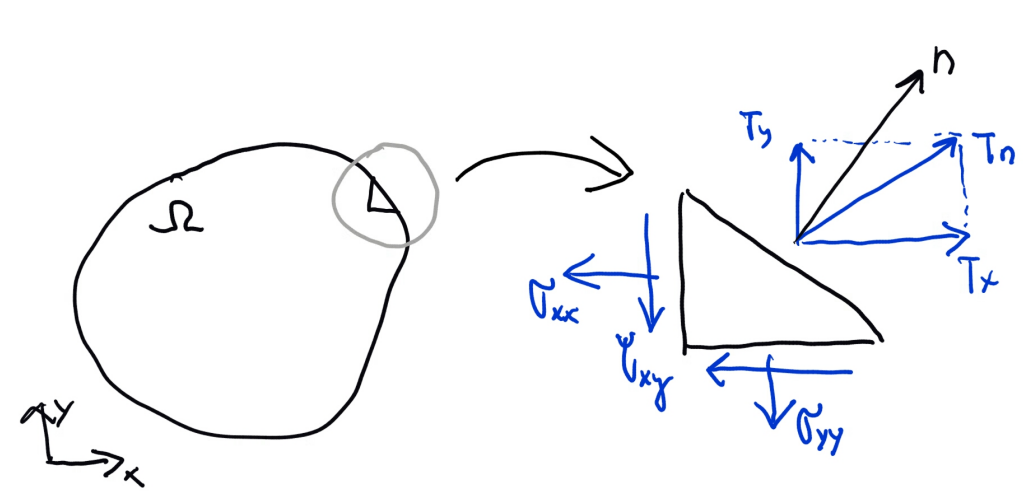
\includegraphics[width=0.5\textwidth]{figs/tractionstressrelation.png}
  \end{center}
  \label{fig:tractionstressrelation}
  \caption{Balance between tractions and stresses in 2D}
\end{figure}

The components of the Cauchy stress tensor at every point in a material satisfy the equilibrium equations (Cauchy’s equlibrium equations). From the conservation of angular momentum follows the symmetry of the stress tensor. Therefore, the stress state of the medium at any point and instant can be specified by only six independent parameters, rather than nine. These may be written
$$
\left[
  \begin{array}{ccc}
    \sigma_{xx} & \tau_{xy} & \tau_{xz}\\
    \tau_{xy} & \sigma_{yy} & \tau_{yz}\\
    \tau_{zx} & \tau_{zy} & \sigma_{zz}
  \end{array}
\right] 
$$
where the elements $\sigma_{xx}, \sigma_{yy}, \sigma_{zz}$ are called the normal stresses (relative to the chosen coordinate system), and $\tau_{yz}, \tau_{xz}, \tau_{xy}$ the shear stresses.

In a static equlibrium, the Cauchy stress components in every material point satisfy the equilibrium equations, see~ref{fig:stressbalance}
\begin{equation}
  \sigma_{ji, j} + F_i = 0
\end{equation}
where we use summation convention over repated indices and $F_i$ are the components of the body force. In a compact tensorial notation we can write the above equation as
\begin{equation}
  \grad\cdot\sigma + F_i = 0
  \label{eq:staticequlibruim3d}
\end{equation}

\begin{figure}
  \begin{center}
    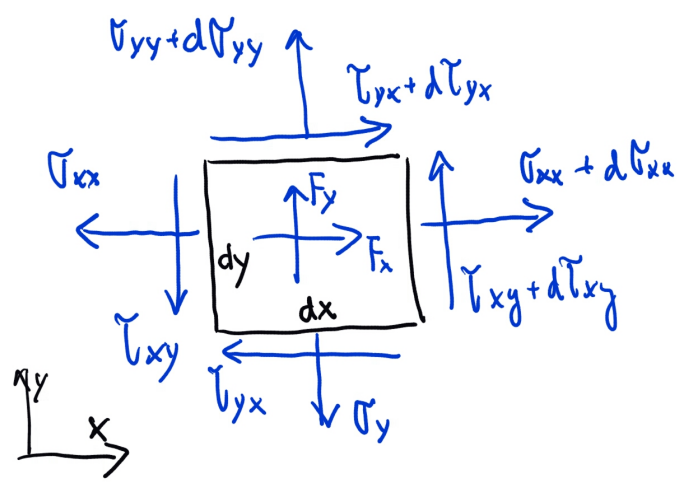
\includegraphics[width=0.5\textwidth]{figs/stressbalance2d.png}
  \end{center}
  \label{fig:stressbalance}
  \caption{Stress balance in 2D}
\end{figure}

\subsection{Constitutive equations}
In this section we present the constituve relations (i.e. relations between stress and strain tensors) for the case of hyperelasticity, which could be defined in terms of strain energy density $W(\mbf{\eps})$, which allows to evaluate stress components as partial derivatives:
$$
\sigma_{ij}=\pard{W}{\eps_{ij}}
$$
For example, the Hooke's law  is defined using following strain energy potential
$$
W(\eps) = \del{1}{2}\eps_{ij}\mbf{C}_{ijkl}\eps_{kl}
$$
where $\mbf{C}$ is forth order elasticity tensor. The equality of mixed derivatives $(\dpd{W}{\eps_{ij}\eps_{kl}} = \dpd{W}{\eps{kl}\eps{ij}})$ and symmetry of stress and strain tensors $\pard{\sigma{ij}}{\eps_{kl}} = C_{ijkl}=C_{jikl}=C_{ijlk}$ imply that there is in general maximum 21 independ components of the elasticity tensor.
In the simplest case, the elasticity tensor for isotropic linear elastic material  can be described by only two parameters: either Lame\'s parameters ($\lambda, \mu$) or more usual parametrs being Young's modulus $E$ and Poisson's ratio $\nu$:
$$
C_{ijkl}=\lambda\delta_{ij}\delta_{kl}+2\mu {1\over 2}[\delta_{ik}\delta_{jl}+
 \delta_{il}\delta_{jk}] \equiv \mbf{C}=\lambda\mbf{1}\otimes\mbf{I}+2\mu\mbf{I}
$$

\subsection{Voight notation}

The Voigt notation is hrequantly used to take advantage of the symmetry of the stress tensor to express the stress tensor as a six-dimensional vector of the following form:
$$
\tilde{\mbf{\sigma}}=
\left[
  \sigma_{x}, \sigma_y, \sigma_z, \tau_{yz}, \tau_{xz}, \tau_{xy}
  \right]^T \equiv
\left[
  \sigma_{xx}, \sigma_{yy}, \sigma_{zz}, \tau_{yz}, \tau_{xz}, \tau_{xy}
  \right]^T
$$

The strain tensor, similar in nature to the stress tensor (both symmetric second-order tensors) can be written in Voight notation as
$$
\tilde{\mbf{\eps }}=
\left[
  \eps_{x}, \eps_y, \eps_z, \gamma_{yz}, \gamma_{xz}, \gamma_{xy}
  \right]^T \equiv
\left[
  \eps_{xx}, \eps_{yy}, \eps_{zz}, 2\eps_{yz}, 2\eps_{xz}, 2\eps_{xy}
  \right]^T
$$

The benefit of using different representations for stress and strain is the scalar invariance
$$
\mbf{\sigma}\cdot\mbf{\eps}=\sigma_{ij}\eps_{ij}=\tilde{\sigma} \tilde{\eps}
$$
Similarly, a three-dimensional symmetric fourth-order tensor can be reduced to a [6,6] matrix.


\subsection {Boundary value problem in small strain elasticity}
\subsubsection{Strong form}

Starting from the equilibrium equations~ref{eq:staticequlibrium3d}, into which we can substitute the constituve equations and strain-displacement relation we obtain the equlibrium equation expressed in terms of displacements:
$$
\pard{}{x_j}\left({C_{ijkl} {1\over 2}(\pard{u_k}{x_l}+\pard{u_l}{x_k})}\right) + F_i = 0
$$
This system of three partial differnetial equations can be solved, provided that appropriate boundary conditions are given. In summary, the strong form is the following:\\
\begin{center}
\fbox{
  \begin{minipage}{8cm}
    Find $\mbf{u}\in R^n$, such that\\[4mm]
    $\pard{}{x_j}\left({C_{ijkl} {1\over 2}(\pard{u_k}{x_l}+\pard{u_l}{x_k})}\right) + F_i = 0 \in \Omega\,$\\[2mm]
    $\mbf{u}=\mbf{\bar{u}} \in \Gamma_u$\\[2mm]
    $\mbf{t}^n_i = C_{ijkl}{1\over 2}(\pard{u_k}{x_l}+\pard{u_l}{x_k})\,n_j = \bar t_i \,\in \Gamma_t$
  \end{minipage}
}
\end{center}

\subsubsection{Weak form}

  By following the method of weighted residuals, we multiply the governing differential equations~\ref{eq:equlibriumequations3d} in residual form by a sutable test functions $\delta\mbf{u}$, satisfying the homogeneous boundary conditions on $\Gamma_u$
  $$
  \int_\Omega \delta\mbf{u} \cdot \left(
  \grad\cdot\mbf{\sigma} + F \right)\ d\Omega = \mbf{0}
  $$
  By applying the Green's formula, we arrive at
  $$
  \int_\Omega\grad\delta\mbf{u}\cdot\mbf{\sigma}\ d\Omega =
  \int_\Omega\delta\mbf{u}\cdot\mbf{F}\ d\Omega + \int_\Gamma\delta\mbf{u}\cdot\mbf{\sigma}\mbf{n}\ d\Gamma
  $$
  Then we can substitute for the stresses and tractions and taking into account the symmetry of stress tensor ($\sigma=C\mbf{\eps})$
  \begin{equation}
  \int_\Omega\grad^s\delta\mbf{u}\cdot\mbf{C}\mbf{\eps}\ d\Omega =
  \int_\Omega\delta\mbf{u}\cdot\mbf{F}\ d\Omega + \int_\Gamma\delta\mbf{u}\cdot\mbf{t}\ d\Gamma
  \label{weakform3d}
  \end{equation}
  Or, equaivalently using Voight's notation
  \begin{equation}
  \int_\Omega\delta\tilde{\eps}^T\tilde{\mbf{D}}\tilde{\mbf{\eps}}\ d\Omega =
  \int_\Omega\delta\mbf{u}^T\mbf{F}\ d\Omega + \int_\Gamma\delta\mbf{u}^T\mbf{t}\ d\Gamma
  \label{eq:weakformvoight}
  \end{equation}
  
  Note: this is equaivalent to the principle of virtual displacements. For hyperelastic material, the weak form is identical to the principle of minimum potential energy.

  
\subsection{Finite element discretization}
Let us consider discretization of the problem domain $\Omega$ into set of nonoverlapping subdomains $\Omega_e$, called elements.
Next we will consider the approximation of the unknown displacement field, defined on individual subdomains. Note that the approximation is not arbitrary:
\begin{itemize}
  \item The weak form kontains only first derivatives of the unknown and test functions, thus only $C^0$ continuity is required.
\end{itemize}
The element approxiamtion of the arbitrary function $f$ has the form
$$
f = \sum N_j(\mbf{x})r_j  = \mbf{N}\mbf{r}
$$
where $N_j$ are so called shape or approximation functions and $r_j$ are nodal values.
Note that for the approximation functions to be interpolatory, the shape functions have to satisfy Kronecker-delta property, i.e., $N_j(\mbf{x}_i)=\delta_{ij}$, where $\mbf{x}_i$ is the position vector of the i-th node. Also, the shape functions have to satisfy the condition $\sum N_i=1$, which follows from the requirement to approximate the constant function.
The required continuity of element approximations have to be satisfied. This is typically achieved by enforcing the continuity at the nodal points.
In our case, the approximation of displacements and test functions is
\begin{eqnarray}
  \mbf{u}^e&=&\mbf{N}^e(\mbf{x})\mbf{r}^e\\
  \delta\mbf{u}^t&=&\mbf{N}^e(\mbf{x})\delta\mbf{r}^e
\end{eqnarray}

We will use the weak form~\ref{weakform3d}, which using Voight's notation has the form
$$
  \int_\Omega\grad^s\delta\mbf{u}\cdot\mbf{C}\mbf{\eps}\ d\Omega =
  \int_\Omega\delta\mbf{u}\cdot\mbf{F}\ d\Omega + \int_\Gamma\delta\mbf{u}\cdot\mbf{t}\ d\Gamma
$$

  We will need also the derivatives of the displacement and test functions
  \begin{eqnarray}
  \tilde{\eps}^e = = \mbf{B}^e(\mbf{x})\mbf{r}^e\\
  \delta\tilde{\eps}^e&=&\mbf{B}^e(\mbf{x})\delta\mbf{r}^e
\end{eqnarray}
where $B^e$ matrix contains the first partial derivatives of the shape functions. 
By substiituting into the weak form~\ref{eq:weakformvoight} we obtain
\begin{equation}
  \sum_e \delta\mbf{r}^{e,T}
  \left[
    \underbrace{\int_{\Omega^e} \mbf{B}^{e,T}\tilde{\mbf{D}}^e\mbf{B}^e\mbf{r}^e\ d\Omega}_{\mbf{K}^e}\mbf{r}^e-\underbrace{\int_{\Omega}\mbf{N}^{e,T}\mbf{F}\ d\Omega}_{\mbf{f}^e_\Omega} - \underbrace{\int_{\Gamma_t}\mbf{N}^{e,T}\bar{\mbf{t}}\ d\Gamma}_{\mbf{f}^e_\Gamma}
    \right] = \mbf{0}
\end{equation}

After introducing a mappig between element displacement vectors $\mbf{r}^e$, nodal vectors of test function values $\delta\mbf{r}$ and their global counterparts $\hat{\mbf{r}}, \delta\hat{\mbf{r}}$ one can obtain
\begin{equation}
  \delta\hat{\mbf{r}}^{T}
  \left[
    \hat{\mbf{K}}\hat{\mbf{r}}-\hat{\mbf{f}}_\Omega - \hat{\mbf{f}}_{\Gamma}
    \right] = \mbf{0}
\end{equation}
By taking into account that the test fuctions are arbitrary (i.e. $\delta\hat{\mbf{r}}\ne\mbf{0}$), one finnaly obtains the following set of linear algebraic equations for unknonwn nodal displacements $\hat{\mbf{r}}$:
\begin{equation}
    \hat{\mbf{K}}\hat{\mbf{r}}=\hat{\mbf{f}}_\Omega + \hat{\mbf{f}}_{\Gamma}
\end{equation}



\chapter{Solution procedures}
\section{Transient incompressible flow\\PFEM Algorithm}
\subsection{Lagrangian governing equations of incompressible fluid}
The Particle finite element method (PFEM) is based on the Lagrangian form of the Navier-Stokes equation for incompressible Newtonian fluids. Assuming the density does not change in time for an incompressible fluid, the continuity equation reduces to zero requirements for the divergence of the velocity. The Navier-Stokes equations take the form
\begin{eqnarray}
\rho\pard{\mbf{u}}{t} &=& \rho\mbf{b} + \nabla\cdot\mbf{\sigma} \label{eq:navier-stokes2}\;,\\
\nabla\cdot\mbf{u} &=& 0\;. \label{eq:navier-stokes2b}
\end{eqnarray}
For the deviatoric stress in Newtonian fluids a linear dependency of stress tensor and strain rate tensor is adopted and for the Newtonian fluids. Considering the incompressibility of the fluid, the Cauchy stress reads
\begin{equation}\label{eq:stokes}
\mbf{\sigma}=-p\mbf{I} + 2\mu \nabla^s\mbf{u}\;.
\end{equation}
This equation is known as \emph{Stokes' law} and its Cartesian form writes
\begin{equation}
\sigma_{ij}=-p\delta_{ij}+\mu\left(\pard{u_i}{x_j}+\pard{u_j}{x_i}\right)\;.
\end{equation}
\par
Substituting the expression of Cauchy stress from Stokes' law~(\ref{eq:stokes}) into the momentum equation~(\ref{eq:navier-stokes2}) and rewriting gives
\begin{equation}
\rho\pard{\mbf{u}}{t} = \rho\mbf{b} + \mu\nabla^2\mbf{u} - \nabla p\;.\label{eq:momentum}
\end{equation}
\par
The governing equations of the mass~(\ref{eq:navier-stokes2b}) and momentum conservation~(\ref{eq:momentum}) form can be written in the Cartesian form for the individual component $i$ using Einstein summation convention
\begin{eqnarray}
\rho \pard{u_i}{t} &=& - \frac{\partial}{\partial x_i}p+\mu\frac{\partial}{\partial x_j}\left(\frac{\partial u_i}{\partial x_j}\right)+\rho b_i \;, \label{eq:mb}\\
\pard{u_i}{x_i} &=& 0\;.
\end{eqnarray}
The equations are accompanied by a set of standard boundary conditions imposed on the complementary parts of the domain boundary
\begin{eqnarray}
  \tau_{ij}\nu_j - p\nu_i &=& \bar \sigma_{ni} \qquad \mbox{on } \Gamma_{\sigma}\;, \\
  u_i\nu_i &=& \bar u_n \qquad\; \mbox{on } \Gamma_n\;, \\
  u_i\zeta_i &=& \bar u_t \qquad\;\, \mbox{on } \Gamma_t\;,
\end{eqnarray}
where $\nu$ or $n$ denotes the normal direction to the boundary and $\zeta$ or $t$ the tangential one. The bar sign over a quantity $\bar x$ stands for its prescribed value.

\subsection{Time discretization}
For the time discretization of the momentum equation, a general trapezoid rule can be adopted. Using this rule, the time derivative of a generic function $\phi$ can be approximated by following equation
\begin{equation}
[\phi(x,t)]^{n+\theta} = \theta\phi(x,t^{n+1})+(1-\theta)\phi(x,t^n)=\theta\phi^{n+1}+(1-\theta)\phi^n\;.
\end{equation}
Rewriting the time derivative on the left hand side of the momentum balance~(\ref{eq:mb}) as a finite difference in time and applying the trapezoidal rule on the right hand side, we obtain
\begin{equation}\label{eq:momentum-general}
  \rho\pard{u_i}{t} \approx \rho\frac{u^{n+1}_i-u^n_i}{\Delta t}= \left[ - \frac{\partial}{\partial x_i}p+\mu\frac{\partial}{\partial x_j}\left(\frac{\partial u_i}{\partial x_j}\right)+\rho b_i\right]^{n+\theta}\;.
\end{equation}
The parameter $\theta$ can take values from the interval $[0,1]$.  The approximation is considered as a weighted average of the derivative values in the time step $n$ and $n+1$. Using a specific value of the $\theta$ parameter, well-known methods can be recovered: The explicit Euler method $\theta=0$, the backward Euler for $\theta=1$ or the Crank-Nicolson method $\theta=1/2$. The current implemantation of PFEM allows the use of explicit and backward (implicit) method.

\subsection{Fractional step scheme}
Beside the three velocity components, the discretized momentum balance equations~(\ref{eq:momentum-general}) for a three dimensional case includes pressure as a coupling variable. A possible approach to decouple them is the application of so-called \emph{fractional step method}. The main idea of this method consists in introducing an intermediate velocity as supplementary variable and splitting the momentum equation. The modification introduced by R.Codina~\cite{Codina01} splits the the discretized time step is split into two sub-steps. The implicit part of the pressure is avoided and assigned to the second step.
\begin{equation}
  \pard{u_i}{t} \approx \frac{u^{n+1}_i-u^n_i}{\Delta t}=\frac{u^{n+1}_i-u^*_i+u^*_i-u^n_i}{\Delta t}= \left[ - \frac{1}{\rho}\frac{\partial}{\partial x_i}p+\frac{\mu}{\rho}\frac{\partial}{\partial x_j}\left(\frac{\partial u_i}{\partial x_j}\right)+b_i\right]^{n+\theta}\;.
\end{equation}
where the intermediate velocity $u^*_i$ is introduced. Splitting the equation in the following manner gives the expression for the unknown velocities
\begin{eqnarray}\label{rce:uistar}
    u^*_i &=& u^n_i+b_i\Delta t - \frac{\Delta t}{\rho}\pard{}{x_i}\gamma p^n+\frac{\Delta t\mu}{\rho}\pard{}{x_j}\left(\pard{u^{n+\theta}_i}{x_j}\right)\;,\\
    u^{n+1}_i &=& u^*_i- \frac{\Delta t}{\rho}\pard{}{x_i}(p^{n+1}-\gamma p^n)\;. \label{eq:uin1}
\end{eqnarray}

The pressure split is here introduced by the new parameter $\gamma$ defining the amount of splitting and can take values from 0 to 1. The body loads are considered to be constant over time step.
\par
In a similar way, the fractional step method is applied on the mass conservation equation. Here, the time derivative of density would be approximated. As we examine an incompressible flow, whose density does not change in time, merely the intermediate velocity term is incorporated in the divergence of the velocity.
\begin{equation}
  \pard{(u^{n+1}_i-u^*_i+u^*_i)}{x_i} = 0 \;,
\end{equation}
which can be decomposed into two sub-equations

\begin{eqnarray}\label{rce:mass}
	\pard{u^*_i}{x_i} &=& 0 \\
      \pard{(u^{n+1}_i-u^*_i)}{x_i} &=& 0\;.
\end{eqnarray}

By substituting for the velocity difference into the equation~(\ref{eq:uin1}) we obtain
\begin{equation}
\pard{}{x_i}(u^{n+1}_i - u^*_i) = \pard{}{x_i}\left(-\frac{\Delta t}{\rho}\pard{}{x_i}(p^{n+1}-\gamma p^n)\right)\;.
\end{equation}
Now we can sum the separated mass equations together. This operation gives the coupled mass-momentum equation
\begin{equation}
  \pard{u^*_i}{x_i} - \frac{\Delta t}{\rho}\frac{\partial^2}{\partial x^2_i}(p^{n+1}-\gamma p^n) = 0\;.
\end{equation}
The final set of equations reads
\begin{eqnarray}
u^*_i  &=& u^n_i+b_i\Delta t - \frac{\Delta t}{\rho}\pard{}{x_i}\gamma p^n+\frac{\Delta t\mu}{\rho}\pard{}{x_j}\left(\pard{u^{n+\theta}_i}{x_j}\right)\;,\\
\frac{\partial^2}{\partial x^2_i}(p^{n+1}) &=& \frac{\rho}{\Delta t}\pard{u^*_i}{x_i}+\frac{\partial^2}{\partial x^2_i}(\gamma p^n)\;, \\
u^{n+1}_i &=& u^*_i- \frac{\Delta t}{\rho}\pard{}{x_i}(p^{n+1}-\gamma p^n)\;.
\end{eqnarray}
\par
The above PFEM formulation is based on the paper by Idelsohn, O\~nate and Del Pin~\cite{Idelsohn04}. The authors described an approach using arbitrary time discretization scheme and pressure split factor. Their choice of implicit scheme $\theta = 1$ was motivated by better convergence properties, whereas the decision for $\gamma = 0$ leading to greater pressure split was driven by better pressure stabilization.
\subsection{Spatial discretization}
The unknown functions of velocity and pressure are approximated using equal order interpolation for all variables in the final configuration
\begin{eqnarray}
u_i&=&\mbf{N}^T(X,t)\mbf{U}_i\\
p&=&\mbf{N}^T(X,t)\mbf{P} \;.
\end{eqnarray}
By applying the Galerkin weighted residual method on the splitted governing equations, following system of linear algebraic equations is obtained 
\begin{eqnarray}
\mbf{M}\mbf{U}^* &=& \mbf{M}\mbf{U}^n + \Delta t\mbf{F} - \frac{\Delta t\mu}{\rho}\mbf{K}\mbf{U}^{n+\theta}\;,\label{eq:systemA} \\
\mbf{L}\mbf{P}^{n+1} &=&\frac{\rho}{\Delta t}\left(\mbf{G}^T\mbf{U}^*-\hat{\mbf{U}}\right) \;, \label{eq:systemB} \\
\mbf{M}\mbf{U}^{n+1} &=& \mbf{M}\mbf{U}^* - \frac{\rho}{\Delta t}\mbf{G}\mbf{P}^{n+1} \;.\label{eq:systemC}
\end{eqnarray}
\par
The matrix $\mbf{M}$ denotes the mass matrix in a lumped form, whereas the vector $\mbf{F}$ stands for the load vector. The matrix $\mbf{G}$ represents the gradient operator, which is the transposition of the divergence operator denoted simply as $\mbf{G}^T$. Matrices $\mbf{K}$ and $\mbf{L}$ are build in a similar way however noted differently. Both mean the Laplacian operator. Due to its common use in computational mechanics, the classical notation of the stiffness matrix $\mbf{K}$ is used. Prescribed velocity components are enclosed in vector $\hat{\mbf{U}}$.
\par
In each computational time step, an iteration is performed until the equilibrium is reached. Depending on the value of $\theta$ used, the equation system for the components of the auxiliary velocity $U^*_i$~(\ref{eq:systemA}) can be solved either explicitly $\theta = 0$ or implicitly $\theta \neq 0$. Then, the calculated values of the auxiliary velocity are used as input for the pressure computation~(\ref{eq:systemB}). The last system of equations~(\ref{eq:systemC}) determines the velocity values at the end of the time step, taking auxiliary velocities and pressure or pressure increments into account.
\par
Let us summarize the iterative step. The position of the particles at the end of the previous time step is known, as well as the the value of the velocity $u^n$ and pressure $p^n$. The set of governing equations is build up for the unknowns at the end of the solution step $\theta^{n+1}$, however based on the geometry of the previous step. The changes in the position are neglected. Once the convergence is reached, the final position is computed from the old one modified by the displacement due to obtained velocity. After that, solution can proceed to the next time step.

\chapter{Elements}
\chapter{Constitutive Equations}
The purpose of this chapter is to present the theoretical backgroung
of some handy general purpose theories and algorithms, that are provided in oofem in the
form of general material base classes. They can significantly
facilitate the implementation of particular material models that are
based on such concepts. Typical example can be a general purpose
plasticity class, that implements general stress return and stifness
matrix evaluation algorithms, based on provided methods for computing
yield functions and corresponding derivatives. Particular
models are simply derived from the base classes, inheriting
common algorithms.


\section{Isotropic damage model}
\label{IsoDamMod}
 In this section, the formulation of an isotropic damage model will be
 described. To cover the various models based on isotropic damage concept,
 a base class IsotropicDamageMaterial is defined first,
 declaring the necessary services and providing the implementation of
 them, which are general. The derived classes then only  implement a particular
 damage-evolution law.

 The isotropic damage models are based on the simplifying assumption
 that the stiffness degradation is isotropic, i.e., stiffness moduli
 corresponding to different directions decrease proportionally and
 independently of direction of loading. Consequently, the damaged
 stiffness matrix is expressed as
 $$
\mbf{D} = (1-\omega)\mbf{D}_e,
 $$
 where $\mbf{D}_e$ is elastic stiffness matrix of the undamaged
 material and $\omega$ is the damage parameter. Initially, $\omega$ is
 set to zero, representing the virgin undamaged material, and the response is
 linear-elastic. As the material undergoes the deformation, the
 initiation and propagation of microdefects decreases the stiffness,
 which is represented by the growth of the damage parameter $\omega$.
 For $\omega = 1$, the stiffness completely disappears.

 In the present context, the $\mbf{D}$ matrix represents the secant
 stiffness that relates the total strain to the total stress
 $$
 \mbf{\sigma}=\mbf{D}\mbf{\varepsilon} = (1-\omega)\mbf{D}_e\mbf{\varepsilon}.
 $$
 Similarly to the theory of plasticity, a loading function $f$ is
 introduced. In the damage theory, it is natural to work in the strain
 space and therefore the loading function is depending on the strain
 and on an additional parameter $\kappa$, describing the evolution of
 the damage. Physically, $\kappa$ is a scalar measure of the
 largest strain level ever reached. The loading function usually has
 the form
 $$
 f(\mbf{\varepsilon}, \kappa) = \tilde\varepsilon(\mbf{\varepsilon}) - \kappa,
 $$
 where $\tilde\varepsilon$ is the equivalent strain, i.e., the scalar
 measure of the strain level.
 Damage can grow only if current state reaches the boundary of elastic
 domain ($f=0$). This is expressed by the following loading/unloading
 conditions
 $$
 f \le 0,\;\;\dot\kappa \ge0,\;\;\dot\kappa f = 0.
 $$
 It remains to link the variable $\kappa$ to the damage parameter
 $\omega$. As both $\kappa$ and $\omega$ grow monotonically, it is
 convenient to postulate an explicit evolution law
 $$
 \omega = g(\kappa).
 $$
 The important advantage of this explicit formulation is that the
 stress corresponding to the given strain can be evaluated directly,
 without the need to solve the nonlinear system of equations.
 For the given strain, the corresponding stress is computed simply by
 evaluating the current equivalent strain, updating the maximum
 previously reached equivalent strain value $\kappa$  and the damage
 parameter and reducing the effective stress according to $\mbf{\sigma}
 = (1-\omega)\mbf{D}_e \mbf{\varepsilon}$.

 This general framework for computing stresses and
 stiffness matrix is  common for all material models of this type.
 Therefore, it is natural to introduce
 the base class for all isotropic-based damage models which provides the general
 implementation for the stress and stiffness matrix evaluation
 algorithms. The particular models then only provide their equivalent
 strain and damage evolution law definitions.
 The base class only declares the virtual services for computing equivalent
 strain and corresponding damage. The implementation of common services
 uses these virtual functions, but they are only declared at
 IsotropicDamageMaterial class level and have to be
 implemented by the derived classes.

 Together with the material model, the corresponding status has to be
 defined, containing all necessary history variables.
 For the isotropic-based damage models, the only history variable is
 the value of the largest strain level ever reached ($\kappa$).
 In addition, the corresponding damage level $\omega$ will be stored.
 This is not necessary because damage can be always computed from
 corresponding $\kappa$.
 The IsotropicDamageMaterialStatus class is derived from
 StructuralMaterialStatus class. The base class represents the
 base material status class for all structural statuses. At
 StructuralMaterialStatus level, the attributes common to all
 ``structural analysis'' material models - the strain and
 stress vectors (both the temporary and non-temporary) are introduced. The
 corresponding services for accessing, setting, initializing, and
 updating these attributes are provided.
 Therefore, only the $\kappa$ and $\omega$ parameters are introduced
 (both the temporary and non-temporary). The corresponding services for
 manipulating these attributes are added and services for context
 initialization, update, and store/restore operations are overloaded, to
 handle the history parameters properly.



\section{Multisurface plasticity driver - MPlasticMaterial class}

In this section, a general multisurface plasticity theory with
hardening/softening is reviewed. The presented algorithms are
implemented in MPlasticMaterial class.



\subsection{Plasticity overview}
Let $\mbf{\sigma},\e, {\rm and}\  \ep$ be the stress, total strain, and plastic strain vectors, respectively.
It is assumed that the total strain is decomposed into reversible elastic and irreversible plastic parts
\begin{equation}
  \e = \e^e + \ep
\end{equation}
The elastic response is characterized in terms of elastic constitutive matrix $\mbf{D}$ as
\begin{equation}
\label{el1}
\mbf{\sigma}=\mbf{D}\e^e = \mbf{D}(\mbf{\varepsilon}-\ep)
\end{equation}
As long as the stress remains inside the elastic domain, the deformation process is purely elastic and the plastic strain does not change.
It is assumed that the elastic domain, denoted as $IE$ is bounded by a composite yield surface. It is defined as
\begin{equation}
IE=\{(\mbf{\sigma},\mbf{\kappa})|f_i(\mbf{\sigma},\mbf{\kappa})<0, \rm{for\ all\ }i\in\{1,\cdots,m\}\}
\end{equation}
where $f_i(\mbf{\sigma},\mbf{\kappa})$ are $m\ge1$ yield functions intersecting in a possibly non-smooth fashion. The
vector $\mbf{\kappa}$ contains internal variables controlling the evolution of yield surfaces (amount of hardening or softening).
The evolution of plastic strain $\ep$ is expressed in Koiter's form. Assuming the non-associated plasticity, this reads
\begin{equation}
\label{epe}
\epd=\sum^{m}_{i=1} \lambda^i \partial_{\mbf{\sigma}}g_i(\mbf{\sigma},\mbf{\kappa})
\end{equation}
where $g_i$ are plastic potential functions. The $\lambda^i$ are referred as plastic consistency parameters, which satisfy the following Kuhn-Tucker conditions
\begin{equation}
\label{ktc}
\lambda^i\ge0,\;f_i\le0,\;{\rm and}\ \lambda^i f_i=0
\end{equation}
These conditions imply  that in the elastic regime the yield function must remain negative and the rate of the plastic multiplier is zero (plastic strain remains constant) while in the plastic regime the yield function must be equal to zero (stress remains on the surface) and the rate of the plastic multiplier is positive.
The evolution of vector of internal hardening/softening variables $\mbf{\kappa}$  is expressed in terms of a general
hardening/softening law of the form
\begin{equation}
\dot{\mbf{\kappa}} = \dot{\mbf{\kappa}}(\sig, \mbf{\lambda})
\end{equation}
where $\mbf{\lambda}$ is the vector of plastic consistency parameters $\lambda_i$.



\subsection{Closest-point return algorithm}
Let us assume, that at time $t_n$ the total and plastic strain vectors and internal variables are known
$$
\{\mbf{\varepsilon}_n, \mbf{\varepsilon}^p_n, \mbf{\kappa}_n\}\  {\rm given\ at}\ t_n
$$
By applying an implicit backward Euler difference scheme to the evolution equations (\ref{el1} and \ref{epe})
and making use of the initial conditions the following discrete non-linear system is obtained
\begin{eqnarray}
\e_{n+1}&=&\e_n+\Delta\e\\
\label{del}
\sig_{n+1}&=&\mbf{D}(\e_{n+1}-\ep_{n+1})\\
\label{dep}
\ep_{n+1}&=&\ep_{n}+\sum\lambda^i\partial_{\sig} g_i(\sig_{n+1}, \mbf{\kappa}_{n+1})
\end{eqnarray}
In addition, the discrete counterpart of the Kuhn-Tucker conditions becomes
\begin{eqnarray}
\label{dktc}
f_i(\sig_{n+1}, \mbf{\kappa}_{n+1}) &=& 0\\
\lambda^i_{n+1} &\ge& 0\\
\lambda^i_{n+1} f_i(\sig_{n+1}, \mbf{\kappa}_{n+1})&=& 0
\end{eqnarray}
In the standard displacement-based finite element analysis, the strain evolution is determined by the displacement increments computed on the structural level. The basic task on the level of a material point is to evaluate the stress evolution generated by strain history.
According to this, the strain driven algorithm is assumed, i.e. that the total strain $\e_{n+1}$ is given.
Then, the Kuhn-Tucker conditions determine whether a constraint is active. The set of active constraints is denoted as $J_{act}$ and is defined as
\begin{equation}
J_{act}=\{\beta\in\{1,\cdots,m\}|f_\beta=0\ \&\ \dot{f}_\beta=0\}
\end{equation}
Let's start with the definition of the residual of plastic flow
\begin{equation}
\label{rpf}
\mbf{R}_{n+1}=-\ep_{n+1}+\ep_{n}+\sum_{j\in J_{act}}\lambda^j_{n+1}\partial_\sigma g_{n+1}
\end{equation}
By noting that total strain $\e_{n+1}$ is fixed during the increment we can express the plastic strain increment using  (\ref{el1}) as
\begin{equation}
\Delta\ep_{n+1} = -\mbf{D}\Delta\sig_{n+1}
\end{equation}
The linearization of the plastic flow residual (\ref{rpf}) yields\footnote{For brevity, the simplified notation is introduced: $f=f(\sig,\mbf{\kappa}),\  g=g(\sig,\  \mbf{\kappa}),\  \mbf{\kappa}=\mbf{\kappa}(\sig,\lambda)$, and subscript $n+1$ is omitted.}
\begin{eqnarray}
\nonumber
&&\mbf{R}+\mbf{D}^{-1}\Delta\sig+\sum\lambda\partial_{\sigma\sigma}g\Delta\sig+\\
&&+\sum\lambda\partial_{\sigma\kappa}g\cdot(\partial_\sigma\kappa\Delta\sig+\partial_\lambda\kappa\Delta\lambda)+\sum\Delta\lambda\partial_{\sigma}g =0
\end{eqnarray}
From the previous equation, the stress increment $\Delta\sig$ can be expressed as
\begin{equation}
\label{dsig}
\Delta\sig=-\mbf{H}^{-1}\left(\mbf{R}+\sum\Delta\lambda\partial_{\sigma}g+\sum\lambda\partial_{\sigma\kappa}g\partial_{\lambda}\kappa\Delta\lambda\right)
\end{equation}
where $\mbf{H}$ is algorithmic moduli defined as
\begin{equation}
\mbf{H}=\left[\mbf{D}^{-1}+\sum\lambda\partial_{\sigma\sigma}g+\sum\lambda\partial_{\sigma\kappa}g\partial_{\sigma}\kappa\right]
\end{equation}
Differentiation of active discrete consistency conditions (\ref{dktc}) yields
\begin{equation}
\label{ddyc}
\mbf{f}+\partial_{\sigma}\mbf{f}\Delta\sig+\partial_{\kappa}\mbf{f} (\partial_\sigma\kappa\Delta\sig+\partial_\lambda\kappa\Delta\lambda) =0
\end{equation}
Finally, by combining equations (\ref{dsig}) and (\ref{ddyc}), one can obtain expression for incremental vector of consistency parameters $\Delta\mbf{\lambda}$
\begin{equation}
\left[\mbf{V}^T\mbf{H}^{-1}\mbf{U}-\partial_{\kappa}\mbf{f}\partial_{\lambda}\mbf{\kappa}\right]\Delta\mbf{\lambda}=\mbf{f}-\mbf{V}^T\mbf{H}^{-1}\mbf{R}
\end{equation}
where the matrices $\mbf{U}$ and $\mbf{V}$ are defined as
\begin{eqnarray}
\mbf{U} &=& \left[\partial_{\sigma}\mbf{g}+\sum\lambda\partial_{\sigma\kappa}g\partial_{\lambda}\kappa\right]\\
\mbf{V} &=& \left[\partial_{\sigma}\mbf{f}+\partial_{\kappa}\mbf{f}\partial_{\sigma}\kappa\right]
\end{eqnarray}

Before presenting the final return mapping algorithm, the algorithm for determination of the active constrains should be discussed. A yield surface $f_{i,n+1}$ is active if $\lambda^i_{n+1} > 0$. A systematic enforcement of the discrete Kuhn-Tucker condition (\ref{dktc}), which relies on the solution of return mapping algorithm, then serves as the basis for determining the active constraints. The starting point in enforcing (\ref{dktc}) is to define the trial set
\begin{equation}
  J^{trial}_{act}=\{j\in\{1,\cdots,m\}|f^{trial}_{j,n+1} > 0\}
\end{equation}
where $J_{act}\subseteq J_{act}^{trial}$. Two different procedures can be adopted to determine the final set $J_{act}$. The conceptual procedure is as follows
\begin{itemize}
 \item
 Solve the closest point projection with $J_{act}=J_{act}^{trial}$ to obtain final stresses, along with $\lambda^i_{n+1},\ i\in J_{act}^{trial}$.
\item
Check the sign of $\lambda^i_{n+1}$. If $\lambda^i_{n+1} <0$, for some $i\in J_{act}^{trial}$, drop the $i-$th constrain from the active set and goto first point. Otherwise exit.
\end{itemize}

In the procedure 2, the working set $J_{act}^{trial}$ is allowed to change within the iteration process, as follows
\begin{itemize}
\item
Let $J_{act}^{(k)}$ be the working set at the k-th iteration. Compute increments $\Delta\lambda^{i,(k)}_{n+1},\ i\in J_{act}^{(k)}$.
\item
Update and check the signs of $\Delta\lambda^{i,(k)}_{n+1}$. If $\Delta\lambda^{i,(k)}_{n+1} < 0$, drop the i-th constrain from the active set $J_{act}^{(k)}$ and restart the iteration. Otherwise continue with next iteration.
\end{itemize}
If the consistency parameters $\Delta\lambda^{i}$ can be shown to increase monotonically within the return mapping algorithm, the the latter procedure is preferred since it leads to more efficient computer implementation.

The overall algorithm is convergent, first order accurate and unconditionally stable.
The general algorithm is summarized in Tab.~\ref{closespointalgo}.

\begin{table}
\label{closespointalgo}
{\small
\begin{enumerate}
\item
  Elastic predictor

  \begin{enumerate}
  \item
 Compute Elastic predictor (assume frozen plastic flow)\\
 $\sig^{trial}_{n+1} = \mbf{D}\left(\e_{n+1}-\ep_{n}\right)$\\
 $f^{trial}_{i,n+1}=f_i(\sig^{trial}_{n+1},\kap_{n}),\ \rm{for}\ i\in\{1,\cdots,m\}$
  \item
 Check for plastic processes
 IF $f^{trial}_{i,n+1}\le 0$ for all $i\in\{1,\cdots,m\}$ THEN:
 \begin{itemize}
\item[]
  Trial state is the final state, EXIT.
 \end{itemize}
 ELSE:
 \begin{itemize}
 \item[]
$J^{(0)}_{act}=\{i\in\{1,\cdots,m\}|f^{trial}_{i,n+1} > 0\}$
 \item[]
$\e^{p(0)}_{n+1}=\ep_n,\ \kap^{(0)}_{n+1}=\kap_n,\ \lambda^{i(0)}_{n+1}=0$
 \end{itemize}
 ENDIF
\end{enumerate}

\item
  Plastic Corrector
  \begin{enumerate}
  \item[(c)]
 Evaluate plastic strain residual
 \begin{itemize}
 \item[]
$\sig^{(k)}_{n+1} = \mbf{D}\left(\e_{n+1}-\e^{p(k)}_{n+1}\right)$
 \item[]
$\mbf{R}^{(k)}_{n+1}=-\e^{p(k)}_{n+1}+\ep_n+\sum\lambda^{i(k)}_{n+1}\partial_{\sigma}g_i$
 \end{itemize}
  \item[(d)]
 Check convergence
 \begin{itemize}
 \item[]
$f^{(k)}_{i,n+1}=f_i(\sig^{(k)}_{n+1},\kap^{(k)}_{n+1})$
 \item[]
if $f^{(k)}_{i,n+1} < TOL$, for all $i\in J^{(k)}_{act}$ and $\Vert\mbf{R}^{(k)}_{n+1}\Vert<TOL$ then EXIT
 \end{itemize}
  \item[(e)]
 Compute consistent moduli
 \begin{itemize}
 \item[]
$\mbf{G}=\left[\mbf{V}^T\mbf{H}^{-1}\mbf{U}-\partial_{\kappa}\mbf{f}\partial_{\lambda}\mbf{\kappa}\right]^{-1}$
 \end{itemize}
  \item[(f)]
 Obtain increments to consistency parameter
 \begin{itemize}
 \item[]
$\Delta\mbf{\lambda}^{(k)}_{n+1}=\mbf{G}\{\mbf{f}-\mbf{V}^T\mbf{H}^{-1}\mbf{R}\}^{(k)}_{n+1}$
 %%\item[]
%%$\bar{\lambda}^{i,(k+1)}_{n+1}=\lambda^{i,(k)}_{n+1}+\Delta\lambda^{i(k)}_{n+1}$
 \item[]
If using procedure 2 to determine active constrains, then update the active set and restart iteration if necessary
 \end{itemize}
  \item[(g)]
 Obtain increments of plastic strains and internal variables
 \begin{itemize}
 \item[]
$\Delta\e^{p(k)}_{n+1}=\mbf{D}^{-1}\left\{\mbf{R}^{(k)}_{n+1}+\sum\Delta\lambda^{i(k)}_{n+1}\partial_{\sigma}g^{(k)}_{n+1}+\sum\lambda^{i(k)}_{n+1}\partial_{\sigma\kappa}g^{(k)}_{n+1}\partial_{\lambda}\kappa\Delta\lambda^{i(k)}_{n+1}\right\}$
 \item[]
$\Delta\kap^{(k)}_{n+1} = \dot{\mbf{\kappa}}(\sig^{(k)_{n+1}}, \mbf{\lambda}^{k}_{n+1})$
 \end{itemize}
  \item[(h)]
 Update state variables
 \begin{itemize}
 \item[]
$\e^{p(k+1)}_{n+1}=\e^{p(k)}_{n+1}+\Delta\e^{p(k)}_{n+1}$
 \item[]
$\kap^{(k+1)}_{n+1}=\kap^{(k)}_{n+1}+\Delta\kap^{(k)}_{n+1}$
 \item[]
$\lambda^{i(k+1)}_{n+1}=\lambda^{i(k)}_{n+1}+\Delta\mbf{\lambda}^{(k)}_{n+1},\ i\in J_{act}$
 \end{itemize}
  \item[(i)]
 Set k=k+1 and goto step (b)
  \end{enumerate}
\end{enumerate}
}
\caption{General multisurface closest point algorithm}
\end{table}



\subsection{Algorithmic stiffness}
Differentiation of the elastic stress-strain relations (\ref{del}) and the discrete flow rule (\ref{dep}) yields
\begin{eqnarray}
  d\sig_{n+1}&=&\mbf{D}\left(d\e_{n+1}-d\ep_{n+1}\right)\\
  d\ep_{n+1}&=&\sum\left(\lambda^i\partial_{\sigma\sigma}gd\sig + \lambda^i\partial_{\sigma\kappa}g\left(\partial_{\sigma}\kap d\sig+\partial_{\lambda}\kap d\lambda^i\right)+d\lambda^i\partial_{\sigma}g\right)
\end{eqnarray}
Combining this two equations, one obtains following relation
\begin{equation}
\label{algrel1}
  d\sig = \mbf{\Xi}_{n+1} \left\{d\e_{n+1}-\sum\lambda^i\partial_{\sigma\kappa}g\partial_{\lambda}\kap d\lambda^i - \sum d\lambda^i\partial_{\sigma}g\right\}
\end{equation}
where $\mbf{\Xi}_{n+1}$ is the algorithmic moduli defined as
\begin{equation}
  \mbf{\Xi}_{n+1}=\left[\mbf{D}^{-1}+\sum\lambda^i\partial_{\sigma\sigma}g+\sum\lambda\partial_{\sigma\kappa}g\partial_{\sigma}\kap\right]
\end{equation}
Differentiation of discrete consistency condition yields
\begin{equation}
  \label{dcc}
  \partial_\sigma f^i d\sig + \partial_\kappa f^i (\partial_\sigma \kap d\sig + \partial_\lambda \kap d\mbf{\lambda}) = 0
\end{equation}
By substitution of (\ref{algrel1}) into (\ref{dcc}) the following relation is obtained
\begin{equation}
  d\mbf{\lambda} = \mbf{G} \left\{\mbf{V}\mbf{\Xi}d\e\right\}
\end{equation}
where matrix $\mbf{G}$ is defined as
\begin{equation}
 \label{gmat}
  \mbf{G}=\left[\mbf{V}^T\mbf{\Xi}\mbf{U}-\partial_{\kappa}\mbf{f}\partial_{\lambda}\mbf{\kappa}\right]^{-1}
\end{equation}
Finally, by substitution of (\ref{gmat}) into (\ref{algrel1}) one obtains the algorithmic elastoplastic tangent moduli
\begin{equation}
  \del{\rm{d}\sig}{\rm{d}\e}\vert_{n+1}=\mbf{\Xi}-\mbf{\Xi}\mbf{U}\left(\mbf{V}\mbf{\Xi}\mbf{U}-[\partial_{\kappa}f][\partial_{\lambda}\kap]\right) \mbf{V}\mbf{\Xi}
\end{equation}



\subsection{Implementation of particular models}

As follows from previous sections, a new plasticity based class has to
provide only some model-specific services. The list of services, that
should be implemented includes (for full reference, please consult
documentation of MPlasticMaterial class):
\begin{itemize}
\item method for computing the value of yield function
  (computeYieldValueAt service)
\item method for computing stress gradients of yield and load
  functions (method computeStressGradientVector)
\item method for computing hardening variable gradients of yield and load
  functions (method computeKGradientVector)
\item methods for computing gradient of hardening variables with
  respect to stress and plastic multipliers vectors
  (computeReducedHardeningVarsSigmaGradient and
  computeReducedHardeningVarsLamGradient methods)
\item method for evaluating the increments of hardening variables due
  to reached state (computeStrainHardeningVarsIncrement)
\item methods for computing second order derivatives of load and yield
  functions (computeReducedSSGradientMatrix and
  computeReducedSKGradientMatrix methods). Necessary only if consistent stiffness is required.
\end{itemize}





\chapter{Boundary conditions}

\phantomsection
\addcontentsline{toc}{chapter}{Bibliography}

\bibliographystyle{plain}
\bibliography{references}

\end{document}


